\chapter{Terminology and Preliminaries}\label{ch:prelim}

\vspace*{-50pt}

\begin{figure}[ht]
        \includegraphics[width=0.35\textwidth, right]{img/gt-ducks.png}
        \captionsetup{textformat=empty,labelformat=blank}
        \caption{Generated with Dall-E. \url{https://labs.openai.com/}. ``Ducks learning graph theory while swimming on a sea sketched in color complex''}
\end{figure}

\epigraph{\itshape ``All we have to decide is what to do with the time that is given to us.''}{J. R. R. Tolkien, \textit{Gandalf} in \textit{Lord of the Rings}}


In this chapter, we will introduce the core definitions used throughout this thesis. 
Most of the definitions of graph theory are taken from \cite{Diekert2005}. 
For definitions in the area of \textit{parameterized complexity}, the book written by Cygan et al. \cite{Cygan2015} gives an excellent introduction.
For standard mathematical notation, the reader is referred to any introductory textbook into discrete mathematics (e.g. \cite{Rosen2012}).

\section{Graph Theory}

If not explicitly stated otherwise, the following definitions are taken from the book \textit{Graph Theory} written by Reinhard Diestel \cite{diestel10}.

\subsection{Basic Terminology}

\begin{definition}[Graph]
    A simple graph is a pair $G = (V, E)$ of two sets where $V$ denotes the vertices and $E \subseteq V \times V$ the edges of the graph.  A vertex $v \in V$ is incident with an edge $e \in E$ if $v \in e$. Two vertices $x, y$ are adjacent, or neighbours, if $\{x,y \} \in E$. By this definition, graph loops and multiple edges are excluded.
    
    A multigraph is a pair $(V, E)$ of disjoint sets together with a map $E \rightarrow V \cup [V]^2$ assigning to every edge either one or two vertices, its ends. Multigraphs can have loops and multiple edges.
    
    We usually denote the vertex set by $V(G)$ and its edge set by $E(G)$.


    % TODO connected 

\end{definition}

Unless stated otherwise, we usually consider only \textit{simple graphs}, but the notion of \textit{multigraphs} gets important when we later talk about the \textit{underlying multigraph} of a \dreg. 

\begin{definition}[Subgraph and Induced Subgraph]
    Let \G and $G' = (V', E')$ be two graphs. If $V' \subseteq V$ and $E' \subseteq E$ then $G'$ is a \underline{subgraph} of $G$. 
    If $G$ is a subgraph of $G'$ and $G'$ contains all the edges to $G$ with both endpoints in $V(G')$, then $G'$ is an \underline{induced subgraph} of $G$ and we write $G' = G[V(G')]$.
\end{definition}


%TODO Quote
\begin{definition}[Degrees]
    Let \G be a graph. The \textit{degree} $d_G(v)$ (shortly $d(v)$ if $G$ is clear from the context) of a vertex $v \in V$ is the number of neighbors of v. We call a vertex of degree $0$ as \underline{isolated} and one of degree $1$ as a \underline{pendant}. If all the vertices of $G$ have the same degree $k$, then $g$ is $k$-regular.
\end{definition}

% TODO Quote e.g. The open neighborhood number of a graph
\begin{definition}[Closed and Open Neighborhoods {\cite{Balakrishnan2012}}]
    Let \G be a (non-empty) graph. 
    The set of all neighbors of $v$ is the \underline{open neighborhood} of $v$ and denoted by $N(v)$; the set $N[v] = N(v) \cup \{v\}$ is the \underline{closed neighborhood} f $v$ in $G$. When G needs to be made explicit, those open and closed neighborhoods are denoted by $N_G(v)$ and $N_G[v]$. 
\end{definition}

\begin{definition}[isomorphic Graphs]
Let \G and $G' = (V', E')$ be two graphs. We call $G$ and $G'$ \underline{isomorphic}, if there exists a bijection $\phi: V \rightarrow V'$ with $\{x, y\} \in E \Leftrightarrow \phi(x)\phi(y) \in E'$ for all  $x,y \in V$. Such a map $\phi$ is called \underline{isomorphism}.

If a graph $G$ is isomorphic to another graph $h$, we denote $G \simeq H$. 
\end{definition}

\begin{definition}[Paths and Cycles]
    A path is a non-empty graph $P = (V,E)$ of the form $V = \bigcup_{i  \in [k]} \{x_i\}$ and $E = \bigcup_{i \in  [k-1]} \{x_ix_{i+1}\}$ where the $x_i$ are distinct. The vertices $x_0$ and $x_k$ are \underline{linked} by $P$ and are called the \textit{ends} of $P$. The \underline{length} of a path is its number of edges and the path on $n$ vertices is denoted by  $P_n$. We refer to a path $P$ by a natural sequence of its vertices: $P = x_0x_1...x_k$. Such a path $P$ is a path between $x_0$ and $x_k$, or a $x_0,x_k$-path.
    If $P = x_0...x_k$ is a path and $k \geq 2$, the graph with vertex set $V(P)$ and edge set $E(P) \cup \{x_kx_0\}$ is a \underline{cycle}. The cycle on $n$ vertices is denoted as $C_n$.
    The \underline{distance} $d_G(v,w)$ from a vertex $v$ to a vertex $w$ in a graph $g$ is the length of the shortest path between $v$ and $w$. If $v$ and $w$ are not linked by any path in $G$, we set $d_G(v,w) = \infty$. Again, if $G$ is clear from the context, we omit the subscripted $G$ and just write $d(v,w)$ instead.
\end{definition}

\subsection{Graph Classes}

A \textit{graph class} is a set of graphs $\mathfrak{G}$ that is closed under isomorphism that is if $G \in \mathfrak{G}$ and a $H \simeq G$ then $H \in \mathfrak{G}$ as well.

\begin{definition}[Graph Parameters]
Let \G be a graph.
An  \underline{independent set} of $G$ is a set of pairwise non-adjacent vertices. 
A \underline{clique} of $G$ is a set of pairwise adjacent vertices. 
A \underline{vertex cover} of $G$ is a subset of vertices containing at least one endpoint of every edge. 
A \underline{dominating set} is a subset $D$ of vertices such that all vertices not contained in are adjacent to some vertex in $D$.
\end{definition}

\begin{graphclass}[r-partite]
    Let $r \geq 2$ be an integer. A Graph $G = (V, E)$ is called \underline{r-partite} if $V$ admits a partition into $r$ classes such that every edge has its ends in different classes: Vertices in the same partition class must not be adjacent. 
    A \textit{$2$-partite} graph is called \underline{bipartite}. 
    
    An $r$-partite graph in which every two vertices from different partition classes are adjacent is called \underline{complete}. For the \underline{complete bipartite graph} on bipartitions $X \uplus Y$ of size $m$ and $n$, we shortly write $K_{m,n}$. 
\end{graphclass}

\begin{graphclass}[Complete]
If all vertices of a graph \G are pairwise adjacent, we say that $G$ is \underline{complete}. 
A complete graph on $n$ vertices is a $K_n$. A $K_3$ is called a \underline{triangle}.
\end{graphclass}


%\begin{definition}[{\cite[IV. Triangulated Graphs]{Berge1966}}]
%    A graph G is called \textit{chordal} (or in the older literature \textit{triangulated}) graphs if for every cycle $c = [p_1,...,p_n,p_1]$ of length $l > 3$ there is an edge of $G$ joining two non-consecutive vertices of c. Such vertices are called chords of the cycle   
%\end{definition}

\begin{graphclass}[Chordal]
For a graph \G, an edge that joins two vertices of a cycle, but is not itself an edge of the cycle is a \underline{chord} of that cycle.

Furthermore, we say $G$ is \underline{chordal} (or \textit{triangulated}) if each of its cycles of length at least four has a chord. In other words, it contains no induced cycle other than triangles.

\end{graphclass}

\begin{graphclass}[Split]
A \underline{split graph} is a graph \G whose vertices can be partitioned into a clique and an independent set.    
\end{graphclass}

%\begin{graphclass}[Bipartite {\cite[p.5]{Bondy2008}}]
%A \textit{\bg} is a Graph G whose vertex set can be partitioned into two subsets X and Y, so that each edge has one end in X and one end in Y. Such a partition (X,Y) is called a \textit{bipartition} of G.
%\end{graphclass}

%\begin{definition}[Perfect Graphs]
    
%\end{definition}

\begin{graphclass}[Planar]

A \textit{plane graph} is a pair $(V,E)$ of finite sets with the following properties:

\begin{itemize}
    \item $V \subseteq \mathbb{R}^2$ (Vertices),
    \vspace{-2mm}
    \item Every edge is an arc between two vertices, 
    \vspace{-2mm}
    \item different edges have different sets of endpoints, and
    \vspace{-2mm}
    \item The interior of an edge contains no vertex and no point of any other edge
\end{itemize}

An embedding in the plane, or \textit{planar embedding}, of an (abstract) graph $G$ is an isomorphism between $G$ and a plane graph $H$. A \textit{plane graph} can be seen as a concrete \textbf{embedding} of the planar graph into the ``plane'' $\mathbb{R}^2$.

\end{graphclass}

\section{Computational Complexity Theory}

Computational complexity investigates the question of how many computational resources are required to solve a specific problem. 
We are about to introduce two of the most important classes of problems in classical complexity theory:

\begin{cc}[The Class \Pt~ {\cite{Arora2006}}]{cc:pnp}

    If we denote \DTIME as the set of decision problems that are solvable in $\mathcal{O}(n^k)$ time by a deterministic Turing Machine, we can define the class \Pt as:

    \[ \mathrm{P} := \bigcup_{k \in \mathbb{N}}(\mathrm{DTIME}(n^k))\]

\end{cc}

\begin{cc}[The Class \NP~ {\cite{Arora2006}}]{cc:pnp}
    A language $L \subseteq \{0,1\}^*$ is in \Pt if there exists a polynomial $p: \mathbb{N} \rightarrow \mathbb{N}$ and a polynomial-time Turing Machine $M$ such that for every $x \in \{0,1\}^*$,

    \[ x \in L \Leftrightarrow \exists u \in \{0,1\}^{p(|x|)} \mathnormal{s.t.~} M(x,u) = 1 \]

    \noindent If $x \in L$ and $u \in \{ 0,1 \}^{p(|x|)}$ satisfy $M(x,u) = 1$, then we call $u$  a \textit{certificate} for $x$.
\end{cc}

\Pt denotes the class of all problems that are \textit{efficiently solvable} whereas \NP contains all problems whose solution can efficiently be verified. Note that $\Pt \subseteq \NP$, but the opposite is unknown.

\subsection{\NPcn}\label{ch:npc}
A major discovery in the early 1970s was the fact that some problems in \NP are \textit{at least as hard as} as any other problem in \NP by reducing them to each other spanning a whole ``web of reductions'' \cite{Arora2006}.
The first results in this area had been published independently by Cook \cite{Cook1971} and Levin \cite{Levin1973} after Karp \cite{Karp1972} had introduced this idea of problem reductions.
The Cook-Levin-Theorem \cite{Cook1971} states that the \SAT is \NPc, which implies that one single algorithm for any of these problems would be enough to efficiently solve all of them. 
For a comprehensive introduction to classical complexity theory, the reader is referred to \cite{Arora2006}.

\begin{definition}[{Reductions, \NP-hardness and \NPcn \cite{Arora2006}}]
We say that a language $A\subseteq \{0,1\}^*$ is \textit{polynomial-time Karp reducible} to a language $B \subseteq \{0,1\}^*$ (denote $A \leq_p B$) if there is a poly-time computable function $f: \{0,1\}^* \rightarrow \{0,1\}^*$ such that for every $x \in \{0,1\}^*$, $x \in A$ if and only if $f(x) \in B$.

\noindent We say that a problem $B$ is \NPh if $A \leq_p B$ for every $A \in \NP$ and $B$ is \NPc if additionally $B \in NP$ holds.
\end{definition}

There are thousands of \NPc problems we do not expect to be solvable in polynomial time.
The famous question of whether $\Pt = \NP$ or not is still one of the biggest open questions in mathematics bountied with one million dollars by the \textit{Clay Mathematical Institute} \cite{Fortnow2021}. 
Most of the domination problems like \dom, \sdom, \tdom are \NPc.

\paragraph{Coping with \NPcn}

Even though we do not expect \NPc problems to have a polynomial-time algorithm, there are some strategies to cope with them. 
We can either give up the exactness of a solution to possibly find fast \textit{approximation algorithms} or abandon the search for a polynomial-time algorithm in favor of finding good \textit{Exact Exponential (EEA) Algorithms} instead.

A third technique is using additional structural parameters of a specific problem instance and therefore \textbf{restricting the input to special cases}. 
This idea lead to the development of \textit{Parameterized complexity}.

\subsection{Definitions in Parameterized Complexity}\label{cha:param}

Introduced by Downey and Fellows \cite{Downey1999a}, parameterized complexity extends the classical theory with a framework that allows a more finely-grained analysis of computationally hard problems. 
The idea is to measure a problem in terms of input size and an additional (structural) parameter $k$. 

We like to find an algorithm that is only exponential in a function $f(k)$, but polynomial in the instance size.
$k$ denotes how difficult the problem is: 

If $k$ is small then the problem can still be considered tractable although the underlying \NPh problem counts as intractable in general.
Therefore $k$ can be seen as a measure of the difficulty of a given instance.
If not marked otherwise, all definitions are taken from \cite{Cygan2015}.

% One more sentence

\begin{definition}[Parameterized Problem]
    A parameterized problem is a $L\subseteq\Sigma^*\times \mathbb{N}$ ($\Sigma$ finite fixed alphabet) for an instance $(x,k)\in \Sigma^*\times \mathbb{N}$, where k is called the \textit{parameter}.

    The \underline{size of an instance} of an instance $(x,k)$ of a parameterized problem is $\abs{(x,k)} = \abs{x} + k$ where the parameter $k$ is encoded in unary by convention.
\end{definition}

\subsection{Fixed-Parameter Tractability}
We say that a problem is \textit{fixed-parameter tractable (fpt)} if problem instances of size $n$ can be solved in $f(k)n^{\mathcal{O}(1)}$ time for some function $f$ independent of $n$. 
Like the class \Pt can be seen as a notion of \textit{tractability} in classical complexity theory, there is an equivalent in parameterized complexity, which we denote as \FPTl (\FPT) and which we can define the following way:

\begin{cc} [The Class \FPT]{cc:fpt}
    A parameterized problem $L\subseteq\Sigma^*\times\mathbb{N}$ is called \textit{fixed-parameter tractable} if there exists an algorithm A (called a \textit{fixed-parameter algorithm}), a computable function $f:\mathbb{N} \rightarrow \mathbb{N}$ and a constant c such that, given $(x,k) \in \Sigma^* \times \mathbb{N}$, the algorithm $\mathcal{A}$ correctly decides whether $(x,k) \in L$ in time bounded by $f(k) \cdot |(x,k)|^c$. The complexity class containing all fixed-parameter tractable problems is called \FPT.
\end{cc}
\subsection{Kernelization}

A kernelization algorithm is a natural and intuitive way to approach problems and can be seen as a preprocessing procedure that simplifies parts of an instance already before the actual solving algorithm is run. 
A visualization of this idea can be seen in \cref{fig:kernelization}.
One can introduce \textit{reduction rules} that iteratively reduce the instance until we are left with a small kernel.   

\begin{definition}[Kernelization and Reduction Rules]
A \textit{kernelization algorithm} or \textit{kernel} is an algorithm $\mathfrak{A}$ for a parameterized problem $Q$ that given an instance $(I,k)$ of $Q$ runs in polynomial time and returns an equivalent instance $(I', k')$ of $Q$. Moreover, we require that $size_{\mathfrak{A}}(k) \leq g(k)$ for some computable function $g:\mathbb{N} \rightarrow \mathbb{N}$.

A \underline{reduction rule} is a function $\phi:\Sigma^* \times \mathbb{N} \rightarrow \Sigma^* \times \mathbb{N}$ that maps an instance $(x,k)$ to an equivalent instance $(x',k')$ such that $\phi$ is computable in time polynomial in $\abs{x}$ and $k$.

A reduction rule is \underline{sound} (or \underline{safe}) if $(I, k) \in Q \Leftrightarrow (I',k') \in Q$.
\end{definition}

We can give a precise definition of the size of the kernel, after a preprocessing algorithm $\mathfrak{A}$ has been executed.
$size_{\mathfrak{A}}$ denotes the largest size of any instance $I$ after $\mathfrak{A}$ has been applied.
We consider the size to be infinite if it cannot be bounded by a function in $k$.

\begin{definition}[Output size of a Preprocessing Algorithm] The output size of a preprocessing algorithms $\mathfrak{A}$ is defined as 

    \[\mathrm{size}_{\mathfrak{A}}(k) = \sup\{\abs{I'} + k': (I',k')= \mathfrak{A}(I,k), I \in \Sigma^* \} \]
\end{definition}

If we bound $\mathrm{size}_{\mathfrak{A}}$ by a polynomial in $k$, we say that the problem admits a \textbf{polynomial kernel}.  
Analogous, if the size after the reduction is only linear $k$, we refer to it as a \textbf{linear} kernel.

% If we first find the kernel to a parameterized problem $Q$ and then solve this kernel using a fast exact exponential time algorithm yields a running time of $|(I,k)|^c + f(k)$ where 

% If there exists a kernelization algorithm for a problem $L$ and an algorithm $\mathfrak{A}$ with any runtime to decide $L$, the problem is in $FPT$ because after the kernelization pre-processing has been applied, the size of the reduced instance is a function merely in $k$ and independent of the input size $n$.

\begin{figure}
    \centering
    
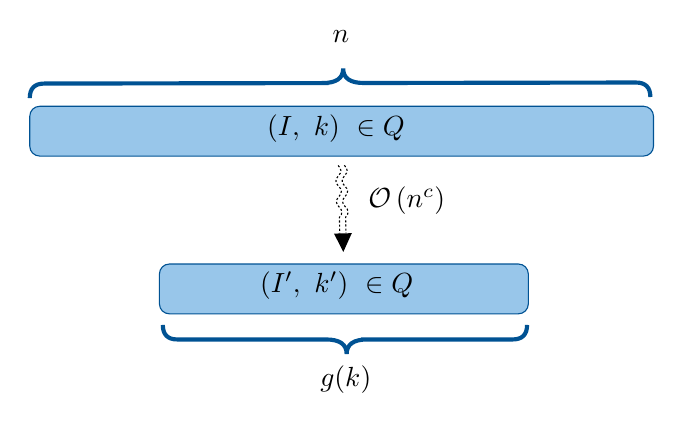
\begin{tikzpicture}[x=0.75pt,y=0.75pt,yscale=-1,xscale=1]
%uncomment if require: \path (0,290); %set diagram left start at 0, and has height of 290
\tikzset{every picture/.style={line width=0.75pt}} %set default line width to 0.75pt        

%Rounded Rect [id:dp2256907851376615] 
\draw  [color={rgb, 255:red, 0; green, 82; blue, 147 }  ,draw opacity=1 ][fill={rgb, 255:red, 152; green, 198; blue, 234 }  ,fill opacity=1 ] (129.8,74.8) .. controls (129.8,72.15) and (131.95,70) .. (134.6,70) -- (425.5,70) .. controls (428.15,70) and (430.3,72.15) .. (430.3,74.8) -- (430.3,89.2) .. controls (430.3,91.85) and (428.15,94) .. (425.5,94) -- (134.6,94) .. controls (131.95,94) and (129.8,91.85) .. (129.8,89.2) -- cycle ;
%Straight Lines [id:da34735862747158275] 
\draw  [dash pattern={on 0.75pt off 0.75pt}]  (281.37,98.46) .. controls (283.08,100.09) and (283.12,101.75) .. (281.49,103.46) .. controls (279.86,105.17) and (279.9,106.83) .. (281.61,108.46) .. controls (283.32,110.09) and (283.36,111.75) .. (281.73,113.46) .. controls (280.1,115.17) and (280.14,116.83) .. (281.85,118.46) .. controls (283.56,120.09) and (283.6,121.75) .. (281.97,123.46) -- (282.08,128.13) -- (282.15,131.13)(278.37,98.54) .. controls (280.08,100.16) and (280.12,101.82) .. (278.49,103.53) .. controls (276.86,105.24) and (276.9,106.9) .. (278.61,108.53) .. controls (280.32,110.16) and (280.36,111.82) .. (278.73,113.53) .. controls (277.1,115.24) and (277.14,116.9) .. (278.85,118.53) .. controls (280.56,120.16) and (280.6,121.82) .. (278.97,123.53) -- (279.08,128.21) -- (279.15,131.21) ;
\draw [shift={(280.87,140.17)}, rotate = 268.63] [fill={rgb, 255:red, 0; green, 0; blue, 0 }  ][line width=0.08]  [draw opacity=0] (8.93,-4.29) -- (0,0) -- (8.93,4.29) -- cycle    ;
%Rounded Rect [id:dp11606859634007116] 
\draw  [color={rgb, 255:red, 0; green, 82; blue, 147 }  ,draw opacity=1 ][fill={rgb, 255:red, 152; green, 198; blue, 234 }  ,fill opacity=1 ] (192.27,150.8) .. controls (192.27,148.15) and (194.42,146) .. (197.07,146) -- (365.2,146) .. controls (367.85,146) and (370,148.15) .. (370,150.8) -- (370,165.2) .. controls (370,167.85) and (367.85,170) .. (365.2,170) -- (197.07,170) .. controls (194.42,170) and (192.27,167.85) .. (192.27,165.2) -- cycle ;
%Shape: Brace [id:dp49500678764931805] 
\draw  [color={rgb, 255:red, 0; green, 82; blue, 147 }  ,draw opacity=1 ][line width=1.5]  (428.8,65.55) .. controls (428.79,60.88) and (426.46,58.55) .. (421.79,58.56) -- (290.81,58.79) .. controls (284.14,58.8) and (280.81,56.48) .. (280.8,51.81) .. controls (280.81,56.48) and (277.48,58.82) .. (270.81,58.83)(273.81,58.82) -- (136.79,59.06) .. controls (132.12,59.07) and (129.79,61.4) .. (129.8,66.07) ;
%Shape: Brace [id:dp39979872340961986] 
\draw  [color={rgb, 255:red, 0; green, 82; blue, 147 }  ,draw opacity=1 ][line width=1.5]  (193.9,175.35) .. controls (193.9,180.02) and (196.23,182.35) .. (200.9,182.35) -- (272.47,182.35) .. controls (279.14,182.35) and (282.47,184.68) .. (282.47,189.35) .. controls (282.47,184.68) and (285.8,182.35) .. (292.47,182.35)(289.47,182.35) -- (362.4,182.35) .. controls (367.07,182.35) and (369.4,180.02) .. (369.4,175.35) ;

% Text Node
\draw (242.9,72.9) node [anchor=north west][inner sep=0.75pt]    {$( I,\ k) \ \in Q$};
% Text Node
\draw (291.67,107.4) node [anchor=north west][inner sep=0.75pt]    {$\mathcal{O}\left( n^{c}\right)$};
% Text Node
\draw (239.5,148.4) node [anchor=north west][inner sep=0.75pt]    {$( I',\ k') \ \in Q$};
% Text Node
\draw (268.5,193.9) node [anchor=north west][inner sep=0.75pt]    {$g( k)$};
% Text Node
\draw (274.5,32.4) node [anchor=north west][inner sep=0.75pt]    {$n$};


\end{tikzpicture}

    \caption{\textit{Kernelization: Reducing an instance $(I,k)$ of size $n$ to a smaller instance $(I', k')$ in polynomial time. The size of the kernel is a function $g(k)$ only dependent on $k$.}}
    \label{fig:kernelization}
\end{figure}

% TODO Do we need this definition?
%\begin{definition}[Equivalent Instance {\cite[p. 18]{Cygan2015}}]
%     This is a test
%\end{definition}

% Relation between Kernelization and FPT
The following \cref{lemma:fptiskernel} shows the relation between the complexity class \FPT and a kernelization algorithm. 
If we find a kernelization algorithm $\mathfrak{A}$ for a (decidable) problem $P$, we immediately obtain an fpt algorithm by first running the $\mathfrak{A}$ on an instance $I$ of $P$ in polynomial time.
Assuming that $P$ can be solved by an algorithm $\mathfrak{M}$ running in time $g(n)$ we can use the fact that the kernel is bounded by a function $f(k)$ and apply $\mathfrak{M}$ on the kernel resulting in a  total running time of the order $\mathcal{O}(g(f(k)) \cdot \mathrm{poly}(n))$ which is fpt.
Surprisingly, also the converse is true:

\begin{lemma}\label{lemma:fptiskernel}
    If a parametrized problem $Q$ is \FPT if and only if it admits a kernelization algorithm.
\end{lemma}

 In \cref{ch:linkern} we will use this and by explicitly constructing a kernel for \psdom, we show membership of the problem in \FPT. 

\subsection{Reductions and Parameterized Intractability}

It is natural to ask whether all hard problems are also fixed-parameter tractable.
It turns out that this is not the case and parameterized complexity answers this question by providing another tool that allows showing that a problem is unlikely to be in \FPT using a different notion of \textit{reductions}.

The idea is to replace the concept of \NP-hardness from the classical setting with a definition of W-hardness for the parameterized framework.
These reductions have to make sure that the equivalent instance is not only created in fpt-time, but must also ensure that the new parameter depends only on the value of the original parameter.

Again there exists a whole hierarchy of classes $\FPT \subseteq \WONE \subseteq \WTWO \subseteq ...$ for which the question whether these inclusions are strict is open.
qwk
Although W[i] spans up a whole hierarchy of complexity classes, in this work we only need the classes \WONE and \WTWO.

Like the class \NP gives strong evidence
must be adjusted

As we can see the class \FPT as some parameterized equivalent for the \P in the classical settings, we might ask wether there is also a notion of \textit{parameterized intractability}.
Are there any problems that are not fixed-p

It turns out that there is whole hierarchy, the so called W-hierarchy.

Before defining these classes, we need a 

% TODO Better formulation!
We can transfer the definitions given in \cref{ch:npc} to the parametrized setting as well. 
We will establish a similar notion for \textit{hardness}

Before defining these classes, we need the notion of a \textit{parameterized reduction} that transfers fixed-parameter tractability.
These reduction preserve \textit{hardness} in the parameterized setting.

\subsubsection{Parameterized Reductions}

\begin{definition}[Parameterized Reduction] Let $A,B\subseteq \Sigma^*\times\mathbb{N}$ two parameterized problems. A \textit{parameter preserving reduction} from $A$ to $B$ is an algorithm that, given an instance $(x,k)$ of $A$, outputs an instance $(x', k')$ of $B$ such that:
    \begin{itemize}
        \item $(x,k)$ is a \textcolor{darkgray}{\textbf{yes instance}} of A \textbf{iff} $(x',k')$ is a \textcolor{darkgray}{\textbf{yes instance}} of B,
        \item $k' \leq g(k)$ for some computable function $g$, and
        \item runs in fpt-time $f(k)\cdot |x|^{\mathcal{O}(1)}$ for some computable function f.
    \end{itemize}
\end{definition}

The following two \cref{lem:cfptr,lem:trans} \cite{Cygan2015} are crucial for proving parameterized intractability and transfer properties, which we had in the classical setting as well.

\begin{lemma}[Closed under fpt-reductions]\label{lem:cfptr}
    If there is a parameterized reduction from $A$ to $B$ and $B \in \FPT$, then $A \in \FPT$, too.
\end{lemma}

\begin{lemma}[Transitivity] \label{lem:trans}
    If there are parameterized reductions from $A$ to $B$ and from $B$ to $C$, then there is a parameterized reduction from $A$ to $C$.
\end{lemma}

Parameterized Complexity class?

We say a problem is \textit{hard}
% TODO. Make better.
We are now ready to define two of the most important classes for fpt.-intractability.

complete, if
We will omit a comprehensive introduction of the W-hierarchy as it is not required for proofing the 

\begin{cc}[The W-hierarchy]{cc:wi}

    \clique is fpt-complete for \WONE.

    \noindent \dom is fpt-complete for \WTWO.

\end{cc}

It is strongly believed that $\FPT \subsetneq W[i]$ and therefore, we do not expect the existence of an algorithm solving any $W[i]$-hard problem in fpt time.

For more background information in parameterized compelxity, we refer the reader to \cite{Cygan2015, Fomin2019}

\chapter{On Parameterized Semitotal Domination}\label{ch:semitotal-domination}

\vspace*{-50pt}

\begin{figure}[ht]
        \includegraphics[width=0.35\textwidth, right]{img/chess.png}
        \captionsetup{textformat=empty,labelformat=blank}
        \caption{Generated with Dall-E. \url{https://labs.openai.com/}. ``Duck playing chess''}
\end{figure}

%\epigraph{\itshape In computer science, parameterized complexity is a framework for studying the complexity of computational problems, in which the complexity of a problem is not just a function of the size of the input, but also a function of one or more additional parameters that describe the problem instance. }{chatGPT, \textit{2022}}
\epigraph{\itshape TODO: Find a nice quote for here!}{chatGPT, \textit{2022}}

In connection with various chessboard problems, the concept of domination can be traced back to the mid-1800s.
For example, De Jaenosch attempted in 1862 to solve the minimum number of queens required to fully cover an $n \times n$-chessboard \cite{Jaenisch1862}. Because of the immense amount of publications related to domination, Haynes, Hedetniemi, and Slater started a comprehensive survey of the literature in 1998 \cite{Haynes1998, Haynes1998b}. 
20 years later, by a series of three more books, Haynes, Henning and Hedetniemi complemented the survey with the latest developments \cite{Haynes2020, Haynes2021, Haynes2022}.

We are now introducing the problems of \dom, \sdom and \tdom and dedicate the rest of the chapter to giving a current status about the complexity status of various graph classes. 

% We will see that most cases mirror each other for the three different problems, but sometimes there seems to be 

% Surprisingly, there are cases where the complexity of \dom and \tdom differes (e)
%If both \dom and \tdom are already hard for a class, we already have a strong assumption that this also holds for \sdom as well.

%Interestingly, most of them mimic each other for one specific class, but there are some exceptions, where this is not the case.

\section{Definition of Domination Problems}

We are now going to define the three most important domination problems for this work: \dom, \sdom and \tdom.
For a specific dominating set $D$, we say that a vertex $d \in D$ is a \textit{dominating vertex} or \textit{dominator}. We say that $d$ \textit{dominates} all of its neighbors.

The \dom problem asks for a subset $D$ of vertices whose set of neighbors covers all the other vertices.
In other words: every vertex $v \notin D$ needs to have at least one neighbor in $D$.

\begin{prb}[\DOM~{\cite[p. 586]{Cygan2015}}]{prb:ds}
    \begin{tabularx}{1.0\textwidth}{>{\hsize=0.30\hsize}X>{\hsize=0.8\hsize}X}
        \textbf{Input} & Graph \G, $k \in \mathbb{N}$\\
        \textbf{Question} & Is there a set {$X \subseteq V$} of size at most $k$ such that ${N[X] = V}$? \\
    \end{tabularx}
\end{prb}

The \tdom problem adds one additional constraint: Every vertex $v \in D$ in the dominating set must also be dominated by some vertex $v' \in D$ which we call the \textit{witness} of $v$.
% TODO: Interesting Property?

\begin{prb}[\TDOM~{\cite[p. 596]{Cygan2015}}]{prb:sds}
    \begin{tabularx}{1.0\textwidth}{>{\hsize=0.30\hsize}X>{\hsize=0.8\hsize}X}
        \textbf{Input} & Graph \G, $k \in \mathbb{N}$\\
        \textbf{Question} & Does there exists a set $X \subseteq V$ with $\abs{X}\leq k$ vertices such that for every $u \in V(G)$ there exists $v \in X$ with $\{u,v\} \in E$ \\
    \end{tabularx}
\end{prb}

Finally, \sdomin was introduced by Goddard, Henning and McPillan \cite{Goddard2014} as a relaxation of \tdomin. 
In this context, we say that $v$ witnesses $v'$ if $v,v' \in D$ and $d(v,v') \leq 2$ for a semitotal dominating set $D$.

\begin{prb}[\SDOM~{\cite{Goddard2014}}]{prb:tds}
    \begin{tabularx}{1.0\textwidth}{>{\hsize=0.30\hsize}X>{\hsize=0.8\hsize}X}
        \textbf{Input} & Graph \G, $k \in \mathbb{N}$\\
        \textbf{Question} & Is there a subset $X \subseteq V$ with $\abs{X} \leq k$ such that ${N[X] = V}$ and for all $d_1 \in X$ there exists another $d_2 \in X$ such that ${d(d_1, d_2) \leq 2}$?\\
    \end{tabularx}
\end{prb}

\begin{figure}
     \begin{equation*}
         \tikzfig{fig/tikz/ds-examples}
     \end{equation*}
    \caption[An example for various dominating sets]{\textit{An example for a dominating set, semitotal dominating set and a total dominating set, where $\gamma(G) < \gamma_{2t}(G) < \gamma_t(G)$ are strict. In the first case, only two vertices suffice to dominate all others. In the second one, we need a witness between $d_1$ and $d_2$ that is at most distance two. In the last case, $d_1$ and $d_2$ both need a neighbor in the total dominating set.}}
    \label{figd:dsexamples}
\end{figure}


\begin{definition}[Domination Parameters]
   The \underline{domination number} in a graph $G$ is the minimum cardinality of a dominating set of $G$, denoted as $\gamma(G)$. 
   The \underline{total domination number} is the minimum cardinality of a total dominating set (tds) of $G$, denoted by $\gamma_t(G)$.
   The \underline{semitotal domination number} is the minimum cardinality of a semitotal dominating set (sds) of $G$, denoted by $\gamma_t(G)$
\end{definition}

% Henning?


Since every total dominating set is also a semitotal dominating set and every semitotal dominating set is also a dominating set , we have the following fact first observed by Goddard and Henning \cite{Goddard2014}. 

\begin{fact}
For every graph $G$ with no isolated vertex, $\gamma(G) \leq \gamma_{t2}(G) \leq \gamma_t(G)$
\end{fact}

We can see that the semitotal domination number $\gamma_{t2}$ is squeezed between the \textit{domination} number and the \textit{total domination} number. It turns out that for some graphs, all of these inequalities can be strict. See \cref{figd:dsexamples} for an example, where $\gamma(G) < \gamma_{t2} < \gamma_t(G)$.

\subsection{Preliminaries}

* Witness
* u pendant ofrom a vertex c if $N(u) = \{w\}$
* domination 

Let $D$ be a dominating set of G and $w \in V(G) \setminus D$. For any neighbor $v \in D \cap N(w)$, we say that $d_1$ \textit{dominates} $w$ For two dominating vertices $d_1, d_2in D$. If 

Definition, dominating number

\section{Complexity Status of \sdom}\label{ch:complexity-status}

% Surprisingly, there are cases where the complexity of \dom and \tdom differes (e)
%If both \dom and \tdom are already hard for a class, we already have a strong assumption that this also holds for \sdom as well.

\section{\hmath $w[i]$-Intractibility}

Now some w[i] hard classes. 

\subsection{Warm-Up: \hmath $W[2]$-hard on General Graphs}

% TODO can we conclude anything for AT Free Graphs?
%% TODO Extend to r-partite

As any \bg with bipartition can be split further into \rpg this results also implies the \wone-hardness of \rpg

